\documentclass[a4paper]{article}
\usepackage[utf8]{inputenc}
\usepackage[russian,english]{babel}
\usepackage[T2A]{fontenc}
\usepackage[left=10mm, top=20mm, right=18mm, bottom=15mm, footskip=10mm]{geometry}
\usepackage{indentfirst}
\usepackage{amsmath,amssymb}
\usepackage[italicdiff]{physics}
\usepackage{graphicx}
\graphicspath{{images/}}
\DeclareGraphicsExtensions{.pdf,.png,.jpg}
\usepackage{wrapfig}

\usepackage{caption}
\captionsetup[figure]{name=Рисунок}
\captionsetup[table]{name=Таблица}
  
\title{\underline{Отчет о выполненой лабораторной работе 1.2.3}}
\author{Антон Хмельницкий, Б01-306}



\begin{document}

\maketitle

\begin{center}
\textbf{\Large Определение моментов инерции твердых тел с помощью трифилярного подвеса}
\end{center}


	\section{Введение}
	\textbf{Цели работы:} измерение момента инерции тел и сравнение результатов с расчетми по теоретиеским формулам; проверка аддитивноски моментов инерции и справедливости формулы Гюйгенса-Штейнера.\\
	\textbf{Оборудование:} трифилярный подвес, секундомер, счетчик числа колебаний, набор тел, момент инерции которых надлежит измерить (диск, стержень, полный цилиндр и другие).
	
	\section{Теоретические сведения}
	
	\begin{wrapfigure}{l}{10cm}
		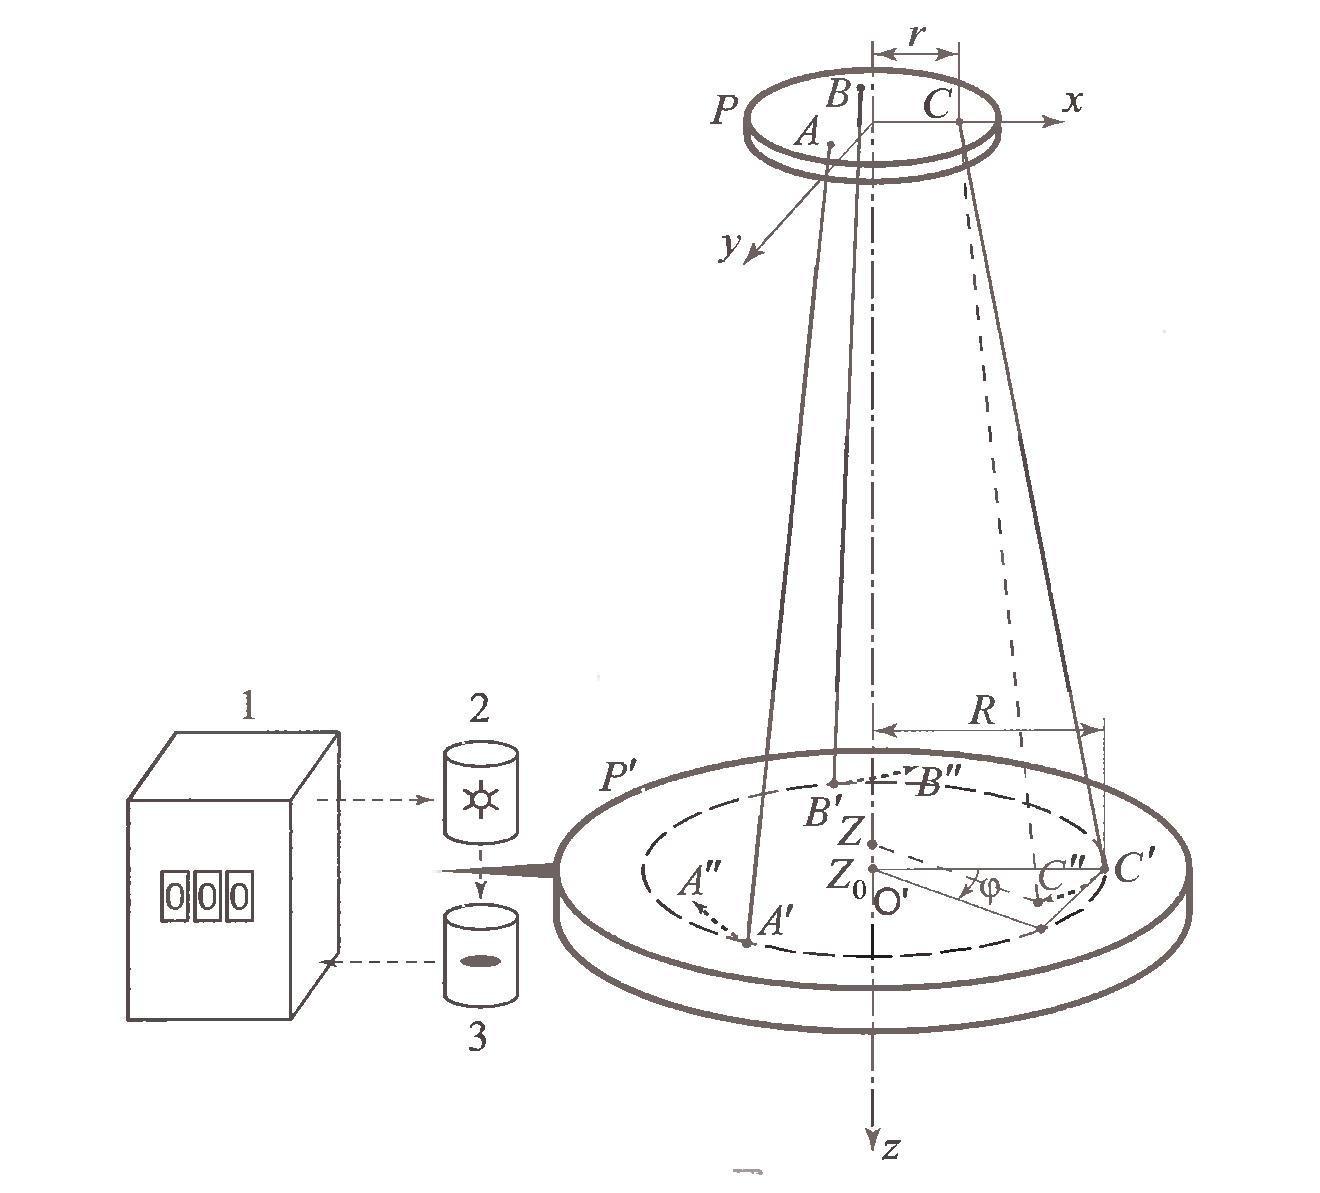
\includegraphics[width=0.95\linewidth]{foto.jpg}
		\caption{Физический маятник}\label{risunok}
	\end{wrapfigure}
	
	Для наших целей удобно использовать устройство, показанное на Рис. \ref{risunok} и называемое трифилярным подвесом. Оно состоит из укрепленной на некоторой высоте неподвижной платформы $P$ и подвешенной к ней на трех симметрично расположеных нитях $AA'$, $BB'$ и $CC'$, вращающейся платформы $P'$. 
	
	Чтобы не вызывать дополнительных раскачиваний, лучше поворачивать верхнюю платформу, укрепленную на неподвижной оси. После поворота верхняя платформа остается неподвижной в течение всего процесса колебний. После того, как нижняя платформа $P'$ оказывается повернутой на угол $\varphi$ относительно верхней платформы $P$, вощникает момент сил, стремящийся вернуть нижнюю платформу в положение равновесия, при котором относительный поворот платформ отсутствует. В результате платформа совершает крутильные колебания.
	
	
	\par Инерционность при вращении тела относительно оси определяется моментом инерции тела относительно этой оси. Момент инерции твердого тела относительно неподвижной оси вращения вычисляется по формуле:
	
	\begin{equation}
		I = \int r^2 dm
	\end{equation}
	
	Здесь $r$ -- расстояние элемента массы тела $dm$ от оси вращения. Интегрирование проводится по всей массе тела $m$.
	
	Если пренебречь потерями энергии на трение о воздух и крепление нитей, то уравнение сохранения энергии при коебаниях можно записать следующим образом:
	
	\begin{equation}\label{moment}
		\frac{I \dot{\varphi^2}}{2} + mg(z_0-z) = E
	\end{equation}
	
	Здесь $I$ -- момент инерции платформы вместе с исследуемым телом, $m$ -- масса платформы с телом, $\varphi$ -- угол поворота платформы от положения равновесия системы, $z_0$ -- координата по вертикали центра нижней платформы $O'$  при равновесии ($\varphi = 0$), $z$ -- координата той же точки при некотором угле поворота $\varphi$. Превый член в левой части уравнения -- кинетическач энергия вращения, второй член -- потенциальная энергия в поле тяжести, $E$ -- полная энергия системы (платформы с телом).
	
	Воспользуемся системой координат $x, y, z$, связанной с верхней платформой, как показано на Рис. \ref{risunok}. Координаты верхнего конца одной из нитей подвеса точки $C$ в этой системе -- $(r, 0, 0)$. Нижний конец данной нити $C'$, находящийся на нижней платформе, при равновесии имеет координаты $(R, 0, z_0)$, а при повороте платформы на угол $\varphi$ эта точка переходит в $C''$ с координатами $(Rcos\varphi, Rsin\varphi, z)$. расстояние между точками $C$ и $C''$ равно длине нити, поэтому, после некоторых преобразований, получаем: 
	
	\begin{center}
		\[ (R\cos\phi - r)^2 + R^2\sin^2\phi + z^2 = L^2 \]
		
		\[ z^2 = L^2 - R^2 - r^2 + 2Rr\cos\phi \approx z^2_{0} - 2Rr(1 - \cos\phi) \approx z^2_{0} - Rr\phi^2 \]
		
		\[ z = \sqrt{z^2_{0} - Rr\phi^2} \approx z_{0} - \frac{Rr\phi^2}{2z_{0}}\]
	\end{center}

	Подставляя $z$ в уравнение \eqref{moment}, получаем:
	
	\begin{equation}
		\frac{1}{2}I\dot{\varphi^2} + mg \frac{Rr}{2z_0}\varphi^2 = E
	\end{equation}
	
	Дифференцируя по времени и сокращая на $\dot\varphi$, находим уравнение крутильных колебаний системы:
	
	\begin{equation}
		I\ddot\varphi^2 + mg\frac{Rr}{2z_0}\varphi^2 = 0
	\end{equation}
		
	Производная по времени от $E$ равна нулю, так как потерями на трение, как уже было сказано выше, пренебрегаем.
	
	Решение этого уравнения имеет вид:
	
	\begin{equation}
		\varphi = \varphi_0 sin \left(\sqrt{\frac{mgRr}{Iz_0}}t + \theta\right)
	\end{equation}

	Здесь амплитуда $\varphi_0$ и фаза $\theta$ колебаний определяются начальными условиями. Период кртуильных полебаний нашей системы равен:
	
	\begin{equation}
		T = 2\pi \sqrt{\frac{Iz_0}{mgRr}}
	\end{equation}

	Из формулы для периода получаем:
	
	\begin{equation}\label{momin}
		I = \frac{mgRrT^2}{4 \pi^2z_0} = kmT^2
	\end{equation}
	\noindent где $k = \frac{gRr}{4\pi^2z_0}$ -- величина, постоянная для данной установки.
	При возбуждении крутильных колебаний маятникообразных движений платформы не наблюдается -- устройство функционирует нормально.
	
	При выводе формул мы предполагали, что потери энергии, связанные с трением, малы, то есть мало затухание колебаний. Это значит, что теоретические вычисления будут верны, если выполняется условие:
 	\begin{equation}
		\tau \gg T
	\end{equation}


 
    \section{Приборы и данные}

    \begin{table}[!h]
    \begin{center}
\begin{tabular}{|c|c|c|}
\hline
                   & Величина & Погрешность \\ \hline
R, радиус (ABC)    & 0,1141   & 0,5 мм      \\ \hline
r, радиус ($A^{'}B^{'}C^{'}$) & 0,0305   & 0,5 мм      \\ \hline
m, масса           & 1,0048   & 0,1 гр      \\ \hline
$L_{0}$            & 2,168    & 1 см        \\ \hline
$z_{0}$            & 2,171    & 1 см        \\ \hline
$M_{\text{диск}}$  & 0,588    & 0,1 гр      \\ \hline
$M_{\text{цил}}$   & 0,982    & 0,1 гр      \\ \hline
$M_{\text{ст}}$    & 1,075    & 0,1 гр      \\ \hline
$D_{\text{диск}}$  & 17,15    & 0,1 мм      \\ \hline
$D_{\text{цил}}$   & 16,71    & 0,1 мм      \\ \hline
$L_{\text{ст}}$    & 20,63    & 0,1 мм      \\ \hline
$D_{\text{ст}}$    & 1,56     & 0,1 мм      \\ \hline
$L_{\text{риска}}$ & 0,6      & 0,1 мм      \\ \hline
$M_{1}$            & 527      & 0,1 гр      \\ \hline
$M_{2}$            & 525,4    & 0,1 гр      \\ \hline
$D_{12}$           & 8,4      & 0,1 мм      \\ \hline
\end{tabular}
\caption{Измеренные размеры тел}
\end{center}
\end{table}
    
    \section{Обработка результатов}

    \subsection{Измерение коэффициента $k$}

    \[k = \frac{gRr}{4\pi^2z_{0}} \approx 3,98 \cdot 10^{-4}\]
    \[\sigma_{k} = k\sqrt{\left( \frac{dk}{dR}\right)^{2} \sigma_{R}^2 + \left(\frac{dk}{dr}\right)^{2}\sigma_{r}^2 + \left(\frac{dk}{dz_{0}}\right)^{2}\sigma_{z_{0}}^2} = k\sqrt{\left( \frac{gr}{4\pi^{2}z_{0}} \right)^2 \sigma_{R}^2 + \left( \frac{gR}{4\pi^{2}z_{0}} \right)^2 \sigma_{r}^2 + \left( \frac{grR}{4\pi^{2}z_{0}^{2}} \right)^2 \sigma_{z_{0}}^2} = 3 \cdot 10^{-9} (\varepsilon_{k} = 0,0008 \%)\]

\subsection{Доказательство аддитивности инерции}
    Используя $I = kmT^2$ получаем рассчитываем моменты инерции для тел на трифилярном подвесе:

\begin{table}[h!]
\begin{center}
\begin{tabular}{|c|c|c|c|c|c|}
\hline
Тела               & Период & $I_{\Sigma}$ экспер., $\text{кг}\cdot\text{м}^2$ & Табличный & $I_{\Sigma}$ расчет., $\text{кг}\cdot\text{м}^2$ & Точность \\ \hline
Платформа          & 4,415  & 0,00765                                  & --        & --                               &  --        \\ \hline
Диск+Платформа     & 3,95   & 0,00989                                  & 0,00216   & 0,00981                          & $0,82\%$ \\ \hline
Цил+Платформа      & 4,24   & 0,0143                                   & 0,00686   & 0,0145                           & $1,38\%$ \\ \hline
Стерж+Платформа    & 3,756  & 0,01169                                  & 0,00383   & 0,01148                          & $1,74\%$ \\ \hline
Диск+Цил+Платформа & 3,996  & 0,01638                                  & --        & 0,01693                          & $2,96\%$ \\ \hline
\end{tabular}
\end{center}
\end{table}

Сравнивая моменты инерции полученные расчетно и экспериментально, убеждаемся что с высокой точностью в $\pm 1\%$  верна аддитивность моментов инерции!

\subsection{Теорема Гюйгенса-Штейнера}

Построим график $I(h^2)$:

\begin{table}[h!]
\begin{center}
\begin{tabular}{|c|c|c|c|}
\hline
№  & $h^2$, $\text{м}^2$ & T, с  & I, $\text{кг}\cdot\text{м}^2$ \\ \hline
1  & 0      & 3,25  & 0,001052516 \\ \hline
2  & 0,25   & 3,264 & 0,001078202 \\ \hline
3  & 1      & 3,285 & 0,001190875 \\ \hline
4  & 2,25   & 3,31  & 0,001325952 \\ \hline
5  & 4      & 3,331 & 0,001440207 \\ \hline
6  & 6,25   & 3,38  & 0,001709613 \\ \hline
7  & 9      & 3,42  & 0,001932454 \\ \hline
8  & 12,25  & 3,5   & 0,002385999 \\ \hline
9  & 16     & 3,55  & 0,00267479  \\ \hline
10 & 20,25  & 3,64  & 0,003204936 \\ \hline
\end{tabular}
\end{center}
\end{table}

\begin{figure}[t]
    \centering
    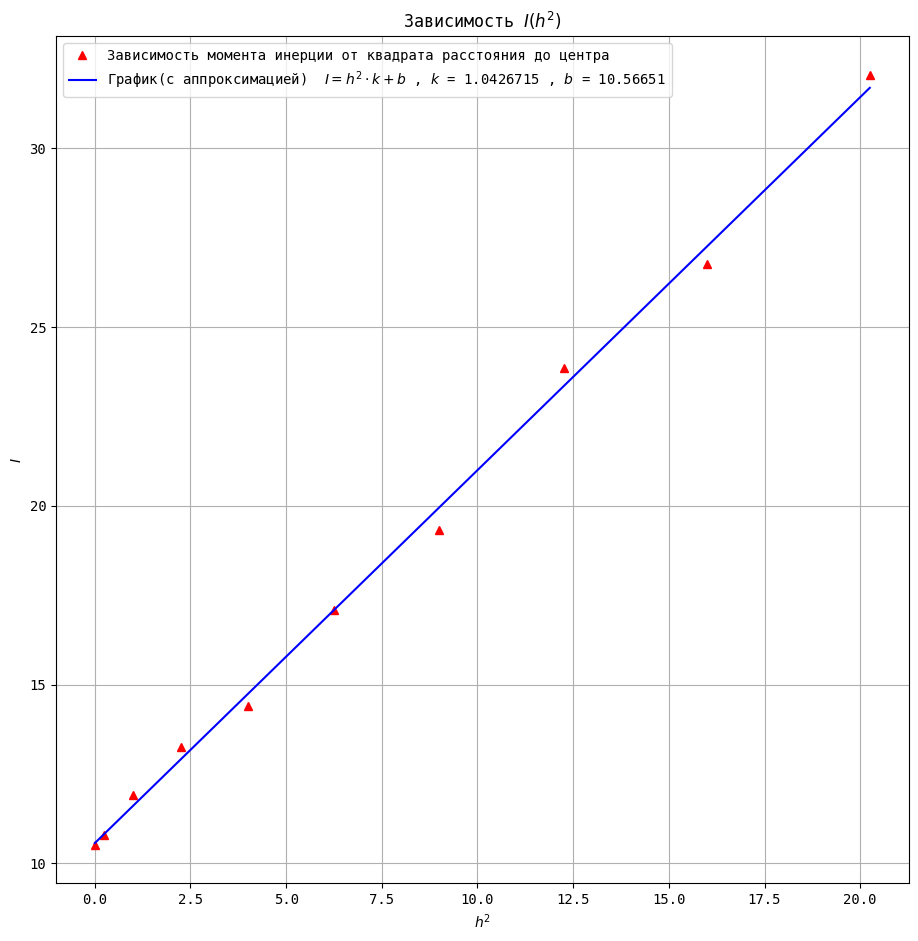
\includegraphics[width=0.8\textwidth]{graphic}
    \caption{Зависимость $I(h^2)$}
\end{figure}

С использованием аппроксимации получаем, что $I = k h^2 + b$ , где k = 1.043 кг и b = 10,57 $\text{кг}\cdot\text{м}^2$.
При этом m = 1.05 кг установки также совпадает с k, а $I(0)$ с погрешностью 0,48\% совпадает с b.

\[k=\frac{\langle xy\rangle-\langle x\rangle \langle y\rangle}{\langle x^2\rangle - \langle x\rangle^2}\approx 1.0426 кг\]

\[\sigma_{k} = \frac{1}{\sqrt{N}}\sqrt{\frac{\langle y^2 \rangle - \langle y \rangle ^2}{\langle x^2 \rangle - \langle x \rangle ^2} - k^2} \approx 0,015 (1,5\%)\]

\[\text{Итого: } k = 1,0426 \pm 0,015 \text{ кг}\]

\newpage
    \section{Выводы}

    С помощью трифилярного подвеса было проведено измерение моментов инерций для различных простых тел: цилиндра, диска, параллилепипеда с высокой точностью $\pm 1\%$, которые подтвердили существующие формулы определения моментов инерций для этих тел.
    Также была экспериментально доказана аддитивность момента инерции, а также теорема Гюйгенса-Штейнера.
\end{document}